\documentclass[12pt]{article}

\usepackage[a4paper,margin=1in]{geometry}
\usepackage{amsmath,amssymb}
\usepackage{newtxtext,newtxmath} % Times-style font
\usepackage{fancyhdr}
\usepackage{listings}
\usepackage{graphicx}
\usepackage{float}
\usepackage{algorithm}
\usepackage{algpseudocode}
\usepackage{xcolor}
\usepackage{booktabs}
\usepackage{array}

\setlength{\textfloatsep}{10pt}
\setlength{\floatsep}{10pt}

\setlength{\parindent}{0pt}
\setlength{\parskip}{5pt}

% Keep entire document at 12 pt
\AtBeginDocument{
    \fontsize{12pt}{14pt}\selectfont
}

\lstdefinestyle{code}{
    language=Python,
    basicstyle=\ttfamily\fontsize{10pt}{12pt}\selectfont,
    breaklines=true,
    breakatwhitespace=false,
    frame=single,
    numbers=left,
    numberstyle=\tiny\color{gray},
    keywordstyle=\color{blue},
    commentstyle=\color{gray},
    stringstyle=\color{green!50!black},
    columns=fullflexible,
    keepspaces=true,
    showstringspaces=false
}

\lstdefinestyle{output}{
    basicstyle=\ttfamily\fontsize{10pt}{12pt}\selectfont,
    breaklines=true,
    breakatwhitespace=false,
    frame=single,
    numbers=none,
    backgroundcolor=\color{gray!4},
    columns=fullflexible,
    keepspaces=true,
    showstringspaces=false
}

% ------------------------------------------------
% Header
% ------------------------------------------------

\pagestyle{fancy}
\fancyhf{}

\fancyhead[L]{Name: Kishan Sahu{\hspace{4cm}}}
\fancyhead[R]{Enrollment No.: P26DS017{\hspace{3.5cm}}}

\renewcommand{\headrulewidth}{0.4pt}
\setlength{\headheight}{15pt}

\begin{document}

% ------------------------------------------------
% TITLE
% ------------------------------------------------

\begin{center}
\textbf{Computer Science and Engineering Department, SVNIT, Surat}\\
\textbf{M.Tech. I -- Semester I}\\
\textbf{Computer Vision and Image Processing (CSCS111/CSDS119)}\\
\textbf{Lab Assignment 4}\\
\textbf{Statistical and Order-Statistic Filtering}
\end{center}

\vspace{0.3cm}

\section{Aim and Objectives}
\begin{enumerate}
    \item To understand the mathematical formulation and operational principles of spatial domain statistical and order-statistic filters.
    \item To implement non-linear order-statistic filters from scratch using vectorized NumPy operations:
    \begin{itemize}
        \item Median Filter
        \item Minimum (Erosion-like) Filter
        \item Maximum (Dilation-like) Filter
        \item Midpoint Filter
        \item Alpha-Trimmed Mean Filter
        \item Percentile / Ranked Order Filters ($25^{\text{th}}$ and $75^{\text{th}}$ percentiles)
    \end{itemize}
    \item To inject synthetic Salt \& Pepper (impulse) and Additive Gaussian noise into standard test imagery (\textit{Cameraman}, $256 \times 256$).
    \item To empirically analyze filter restoration capability across varying spatial neighborhood windows ($3 \times 3$, $5 \times 5$, and $7 \times 7$) and investigate trade-offs between noise suppression and edge preservation.
\end{enumerate}

\section{Mathematical Background}
Order-statistic filters are non-linear spatial filters whose response is based on ranking (ordering) the pixel intensities contained within a localized neighborhood window $S_{xy}$ centered at $(x, y)$.

Let $S_{xy}$ be a square spatial neighborhood of size $k \times k$, comprising $N = k^2$ pixels. Let the pixel values in $S_{xy}$ be sorted in ascending order of intensity:
\begin{equation}
    z_{(1)} \le z_{(2)} \le z_{(3)} \le \dots \le z_{(N)}
\end{equation}
The filtered output $\hat{f}(x, y)$ is computed based on this ranked sequence:

\begin{enumerate}
    \item \textbf{Median Filter:} Selects the median value of the ordered sequence:
    \begin{equation}
        \hat{f}_{\text{med}}(x, y) = \text{median}\{g(s, t) \mid (s, t) \in S_{xy}\} = z_{\left(\frac{N+1}{2}\right)}
    \end{equation}
    The median filter is effective against bipolar impulse (salt-and-pepper) noise because outlier impulse values reside in the extreme tails ($z_{(1)}$ or $z_{(N)}$) and are completely excluded from the output.

    \item \textbf{Minimum Filter (Min Filter):} Selects the lowest intensity value:
    \begin{equation}
        \hat{f}_{\text{min}}(x, y) = \min_{(s, t) \in S_{xy}} \{g(s, t)\} = z_{(1)}
    \end{equation}
    This filter is effective for removing bright salt impulses ($255$), but broadens dark pepper pixels.

    \item \textbf{Maximum Filter (Max Filter):} Selects the highest intensity value:
    \begin{equation}
        \hat{f}_{\text{max}}(x, y) = \max_{(s, t) \in S_{xy}} \{g(s, t)\} = z_{(N)}
    \end{equation}
    This filter eliminates dark pepper impulses ($0$), but broadens bright salt pixels.

    \item \textbf{Midpoint Filter:} Computes the arithmetic average of the two extreme ranked intensities:
    \begin{equation}
        \hat{f}_{\text{mid}}(x, y) = \frac{1}{2} \left[ \min_{(s, t) \in S_{xy}} \{g(s, t)\} + \max_{(s, t) \in S_{xy}} \{g(s, t)\} \right] = \frac{z_{(1)} + z_{(N)}}{2}
    \end{equation}
    The midpoint filter combines order statistics with averaging, performing well for randomly distributed noise with short-tailed probability density functions (such as uniform noise).

    \item \textbf{Alpha-Trimmed Mean Filter:} Trims $d = \lfloor \alpha N \rfloor$ extreme values from both ends of the sorted sequence and computes the arithmetic mean of the remaining $N - 2d$ values:
    \begin{equation}
        \hat{f}_{\alpha}(x, y) = \frac{1}{N - 2d} \sum_{i=d+1}^{N-d} z_{(i)}, \quad \text{where } 0 \le \alpha < 0.5
    \end{equation}
    When $\alpha = 0$, the filter degenerates into an arithmetic mean filter. When $\alpha \to 0.5$ (specifically $d = \frac{N-1}{2}$), it becomes the median filter. It offers an adaptable balance for mixed noise (Gaussian plus impulse noise).

    \item \textbf{Percentile Filter:} Replaces the center pixel with the intensity at a specified percentile $p \in [0, 100]$:
    \begin{equation}
        \hat{f}_{p}(x, y) = z_{(r)}, \quad \text{where } r = \left\lfloor \frac{p}{100}(N-1) \right\rfloor + 1
    \end{equation}
\end{enumerate}

\section{Implementation Details}
The algorithm uses vectorized sliding-window extraction via \texttt{numpy.lib.stride\_tricks.sliding\_window\_view} combined with reflection boundary padding (\texttt{mode='reflect'}). All neighborhood windows across the image grid are simultaneously extracted, reshaped into two-dimensional vectors per pixel, and sorted along the last axis (\texttt{axis=-1}).

\subsection{Image Loading and Noise Generation}
\begin{lstlisting}[style=code]
import cv2
import numpy as np
import matplotlib.pyplot as plt

# Load Cameraman image
img = cv2.imread('Filtering-Cameraman.png', cv2.IMREAD_GRAYSCALE)
print(f"Loaded Cameraman image with dimensions: {img.shape}")
\end{lstlisting}

\begin{lstlisting}[style=output]
Loaded Cameraman image with dimensions: (256, 256)
\end{lstlisting}

\begin{lstlisting}[style=code]
# Noise injection utilities
def add_salt_and_pepper_noise(image, salt_prob=0.03, pepper_prob=0.03):
    noisy = image.copy()
    rnd = np.random.rand(*image.shape)
    noisy[rnd < salt_prob] = 255
    noisy[(rnd >= salt_prob) & (rnd < salt_prob + pepper_prob)] = 0
    return noisy

def add_gaussian_noise(image, mean=0, sigma=20):
    noisy = image.astype(np.float32) + np.random.normal(mean, sigma, image.shape)
    return np.clip(noisy, 0, 255).astype(np.uint8)

np.random.seed(42)
noisy_sp = add_salt_and_pepper_noise(img)
noisy_gauss = add_gaussian_noise(img)

# Display original vs noisy inputs
fig, axes = plt.subplots(1, 3, figsize=(12, 4))
axes[0].imshow(img, cmap='gray')
axes[0].set_title("Original Cameraman")
axes[1].imshow(noisy_sp, cmap='gray')
axes[1].set_title("Salt & Pepper Noise (6%)")
axes[2].imshow(noisy_gauss, cmap='gray')
axes[2].set_title("Gaussian Noise (sigma=20)")
for ax in axes:
    ax.axis('off')
plt.tight_layout()
plt.show()
\end{lstlisting}

\begin{figure}[H]
    \centering
    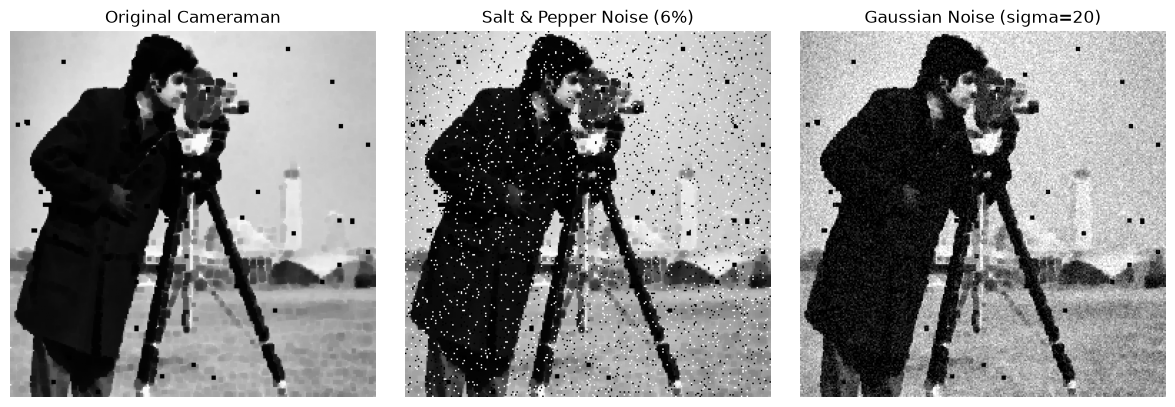
\includegraphics[width=0.95\textwidth]{figures/original_and_noisy.png}
    \caption{Original Cameraman test image and synthetically corrupted inputs: Salt \& Pepper noise ($6\%$ total corruption) and Additive Gaussian noise ($\mu=0, \sigma=20$).}
    \label{fig:original_noisy}
\end{figure}

\subsection{Statistical Order Filter Implementations}
\begin{lstlisting}[style=code]
# Extract and sort sliding window neighborhoods (vectorized via NumPy)
def get_sorted_windows(image, k):
    pad = k // 2
    padded = np.pad(image, pad, mode='reflect')
    windows = np.lib.stride_tricks.sliding_window_view(padded, (k, k))
    return np.sort(windows.reshape(*image.shape, k * k), axis=-1)

# Statistical order filters
def median_filter(sw):
    return sw[..., sw.shape[-1] // 2]

def min_filter(sw):
    return sw[..., 0]

def max_filter(sw):
    return sw[..., -1]

def midpoint_filter(sw):
    return ((sw[..., 0].astype(float) + sw[..., -1].astype(float)) / 2).astype(np.uint8)

def alpha_trimmed_mean_filter(sw, alpha=0.2):
    d = max(1, int(alpha * sw.shape[-1]))  # trim d elements from each tail
    trimmed = sw[..., d : sw.shape[-1] - d]
    return np.clip(trimmed.mean(axis=-1), 0, 255).astype(np.uint8)

def percentile_filter(sw, p):
    idx = int(np.round((p / 100.0) * (sw.shape[-1] - 1)))
    return sw[..., idx]
\end{lstlisting}

\section{Experimental Results}

\subsection{Comparison of Filters on Salt \& Pepper Noise ($3 \times 3$ Kernel)}
The initial evaluation applies all order-statistic filters to the $6\%$ Salt \& Pepper degraded image using a standard $3 \times 3$ window ($k = 3, N = 9$).

\begin{lstlisting}[style=code]
# Apply each filter on Salt & Pepper noisy image (3x3 neighborhood)
k = 3
sw_sp3 = get_sorted_windows(noisy_sp, k)

filters_3x3 = {
    "Median": median_filter(sw_sp3),
    "Min": min_filter(sw_sp3),
    "Max": max_filter(sw_sp3),
    "Midpoint": midpoint_filter(sw_sp3),
    "Alpha-Trimmed (alpha=0.2)": alpha_trimmed_mean_filter(sw_sp3, alpha=0.2),
    "25th Percentile": percentile_filter(sw_sp3, 25),
    "75th Percentile": percentile_filter(sw_sp3, 75)
}

fig, axes = plt.subplots(2, 4, figsize=(16, 8))
axes = axes.ravel()

axes[0].imshow(noisy_sp, cmap='gray')
axes[0].set_title("Noisy Input (Salt & Pepper)")
axes[0].axis('off')

for i, (name, filtered_img) in enumerate(filters_3x3.items(), start=1):
    axes[i].imshow(filtered_img, cmap='gray')
    axes[i].set_title(f"{name} (3x3)")
    axes[i].axis('off')

plt.tight_layout()
plt.show()
\end{lstlisting}

\begin{figure}[H]
    \centering
    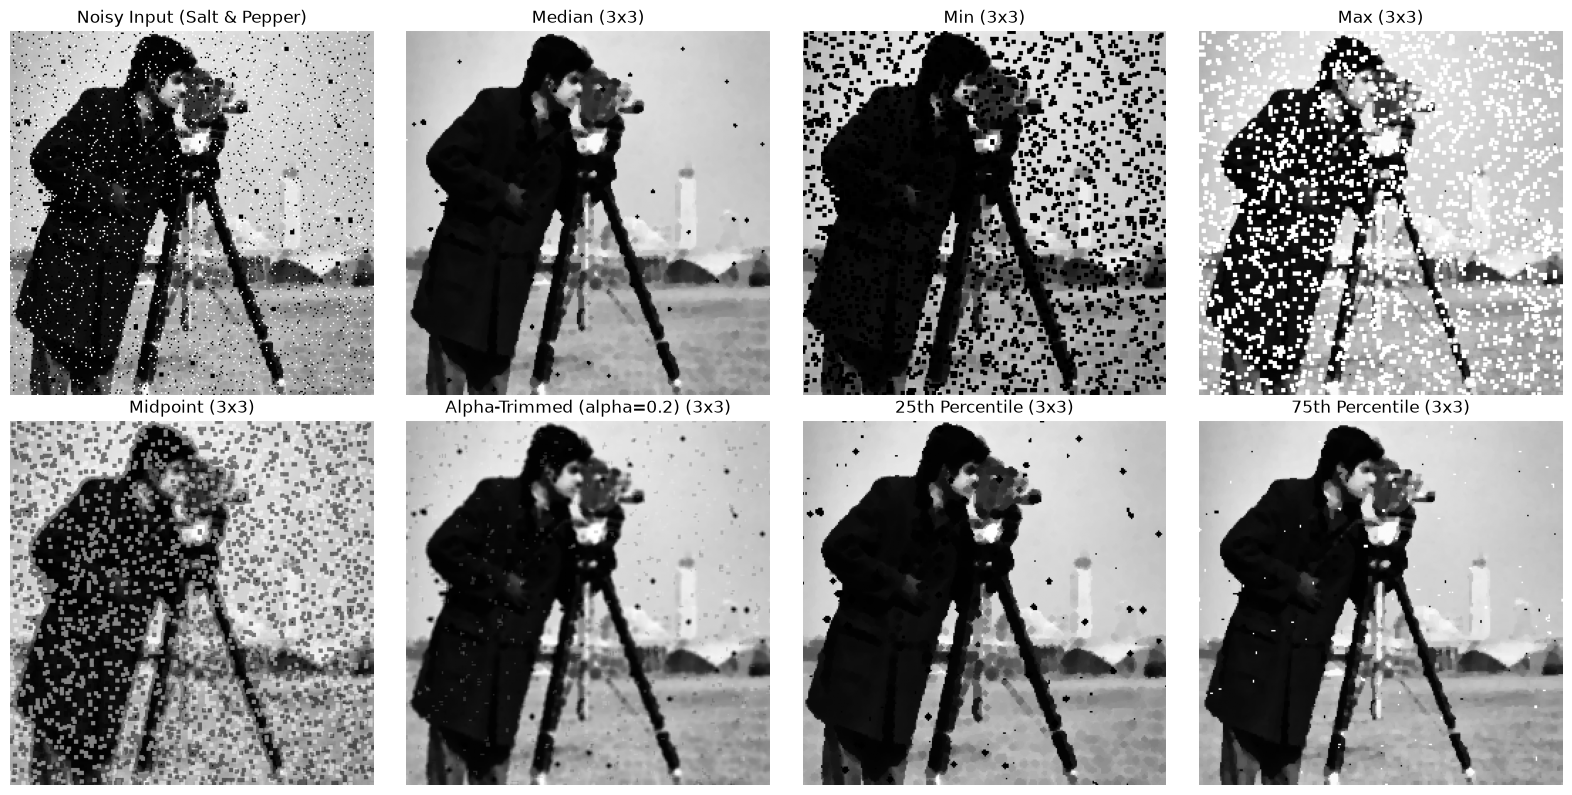
\includegraphics[width=\textwidth]{figures/filters_sp_3x3.png}
    \caption{Comparative performance of statistical order filters on $6\%$ Salt \& Pepper noise with a $3 \times 3$ neighborhood window.}
    \label{fig:filters_sp_3x3}
\end{figure}

\subsection{Impact of Spatial Neighborhood Sizes ($3 \times 3$, $5 \times 5$, and $7 \times 7$)}
The spatial support size $k$ determines the number of samples ($N = k^2$) considered in the ranking. We analyze five filters (Median, Midpoint, Alpha-Trimmed Mean, $25^{\text{th}}$ Percentile, $75^{\text{th}}$ Percentile) across kernel dimensions $k \in \{3, 5, 7\}$.

\begin{lstlisting}[style=code]
# Evaluate filters across neighborhood sizes 3x3, 5x5, and 7x7
sizes = [3, 5, 7]
filter_funcs = {
    "Median": median_filter,
    "Midpoint": midpoint_filter,
    "Alpha-Trimmed": lambda sw: alpha_trimmed_mean_filter(sw, alpha=0.2),
    "25th Percentile": lambda sw: percentile_filter(sw, 25),
    "75th Percentile": lambda sw: percentile_filter(sw, 75)
}

fig, axes = plt.subplots(len(filter_funcs), len(sizes), figsize=(12, 3.2 * len(filter_funcs)))

for r, (fname, ffunc) in enumerate(filter_funcs.items()):
    for c, sz in enumerate(sizes):
        sw = get_sorted_windows(noisy_sp, sz)
        res = ffunc(sw)
        axes[r, c].imshow(res, cmap='gray')
        axes[r, c].set_title(f"{fname} ({sz}x{sz})")
        axes[r, c].axis('off')

plt.tight_layout()
plt.show()
\end{lstlisting}

\begin{figure}[H]
    \centering
    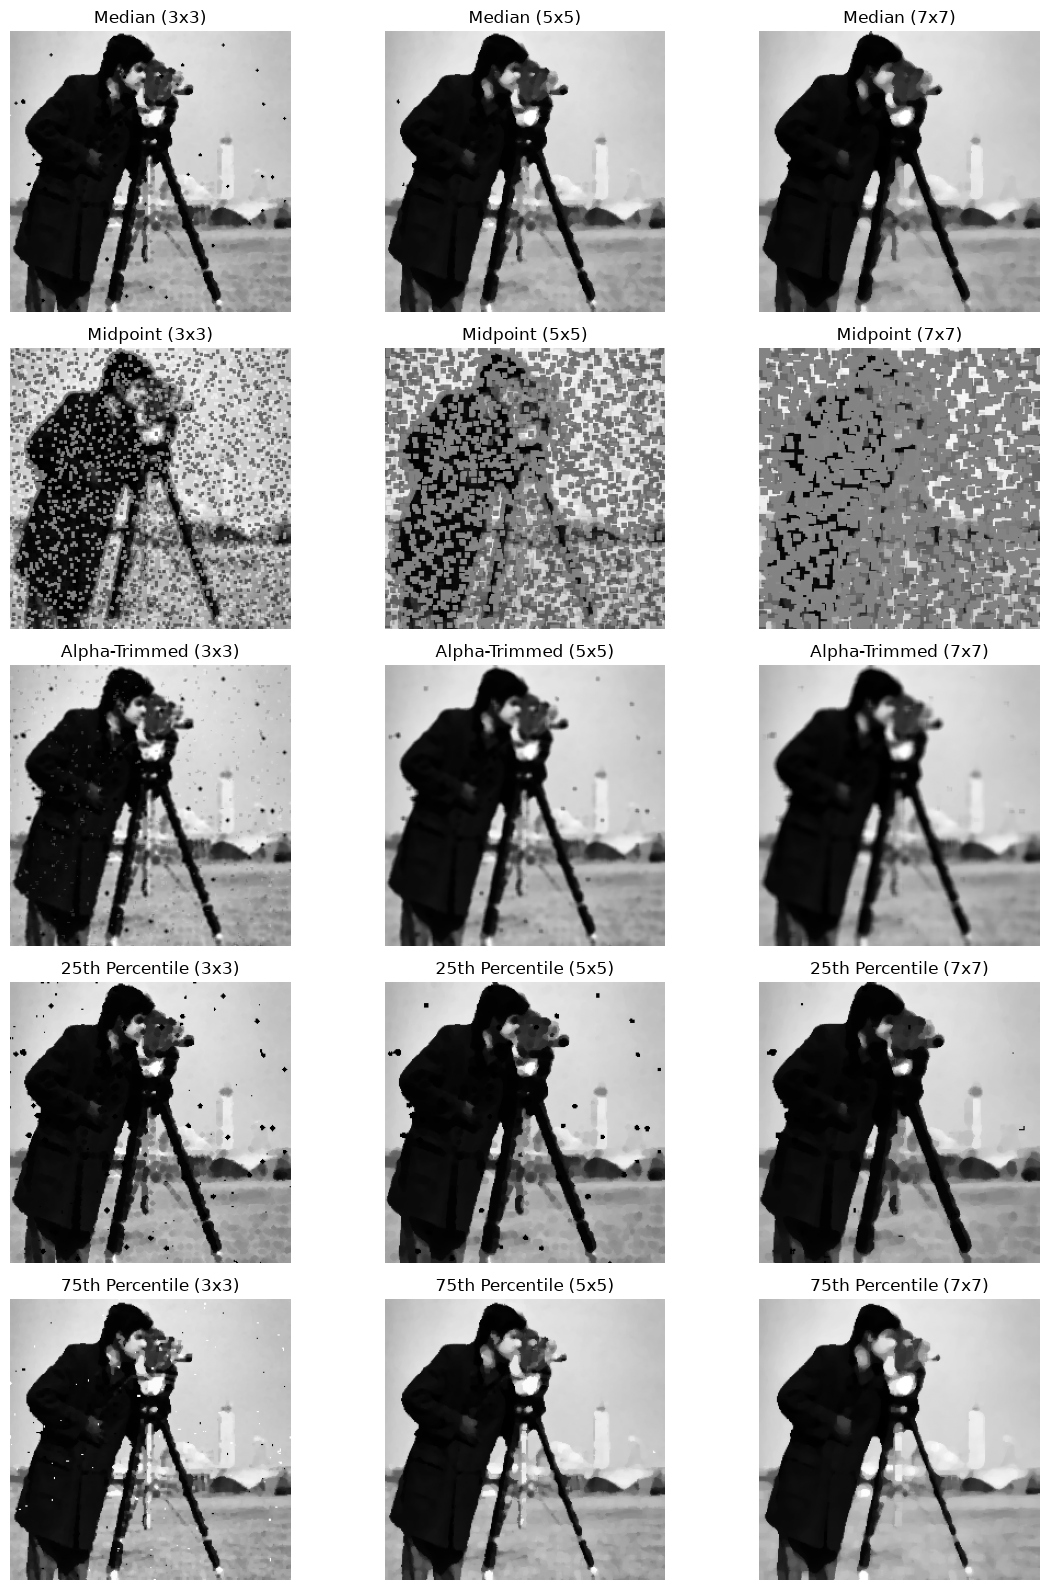
\includegraphics[width=0.88\textwidth]{figures/neighborhood_sizes.png}
    \caption{Effect of neighborhood window sizes ($3 \times 3, 5 \times 5, 7 \times 7$) on noise removal efficiency versus edge detail preservation.}
    \label{fig:neighborhood_sizes}
\end{figure}

\subsection{Evaluation on Additive Gaussian Noise}
To contrast the filtering characteristics between impulse and continuous Gaussian degradation, we evaluate the Median Filter, Midpoint Filter, and Alpha-Trimmed Mean Filter ($\alpha = 0.2$) on the Gaussian corrupted image with $k = 5$.

\begin{lstlisting}[style=code]
# Comparing filter performance on Gaussian noise (5x5 neighborhood)
k = 5
sw_g5 = get_sorted_windows(noisy_gauss, k)

gauss_results = {
    "Noisy Gaussian Input": noisy_gauss,
    "Median Filter (5x5)": median_filter(sw_g5),
    "Midpoint Filter (5x5)": midpoint_filter(sw_g5),
    "Alpha-Trimmed (5x5, a=0.2)": alpha_trimmed_mean_filter(sw_g5, alpha=0.2)
}

fig, axes = plt.subplots(1, 4, figsize=(16, 4))
for ax, (title, out_img) in zip(axes, gauss_results.items()):
    ax.imshow(out_img, cmap='gray')
    ax.set_title(title)
    ax.axis('off')

plt.tight_layout()
plt.show()
\end{lstlisting}

\begin{figure}[H]
    \centering
    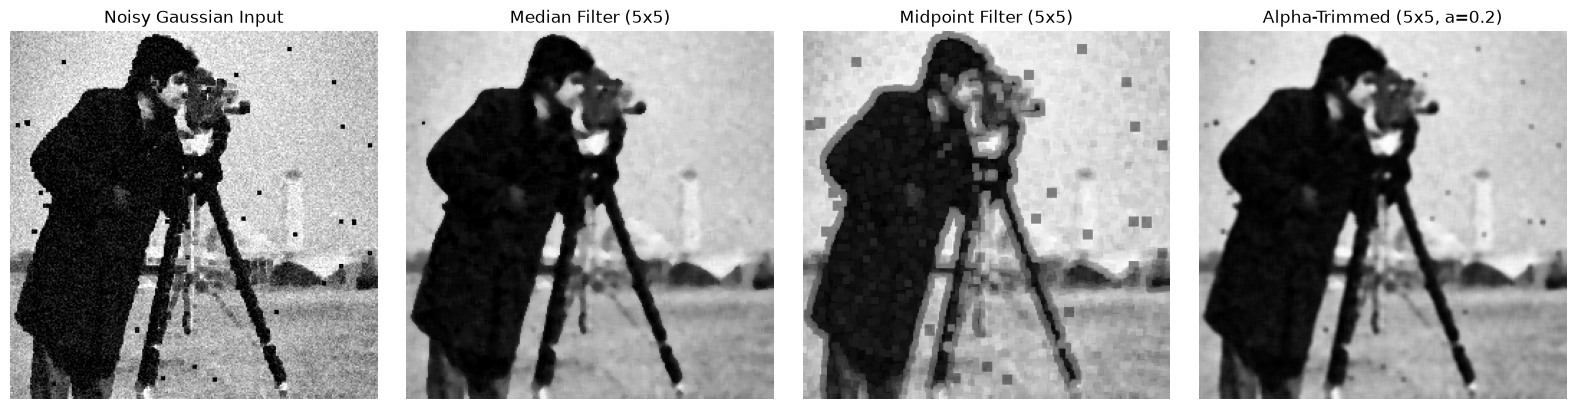
\includegraphics[width=\textwidth]{figures/gaussian_comparison.png}
    \caption{Performance comparison on Additive Gaussian noise ($\sigma=20$) using a $5 \times 5$ neighborhood window.}
    \label{fig:gaussian_comparison}
\end{figure}

\section{Comparative Summary Table}
Table~\ref{tab:filter_comparison} provides a structured synthesis of the theoretical definitions, computational characteristics, optimal applications, and visual behaviors of the investigated statistical order filters.

\begin{table}[H]
\centering
\small
\renewcommand{\arraystretch}{1.25}
\begin{tabular}{p{2.6cm} p{3.2cm} p{1.6cm} p{3.4cm} p{4.2cm}}
\toprule
\textbf{Filter} & \textbf{Mathematical Formula / Rank Index} & \textbf{Complexity} & \textbf{Optimal Noise Environment} & \textbf{Observed Output Characteristics} \\
\midrule
\textbf{Median} & $z_{\left(\frac{N+1}{2}\right)}$ & $O(N \log N)$ & Salt \& Pepper (Impulse) Noise & Completely eliminates isolated impulses; preserves sharp boundaries and fine contours. \\
\textbf{Min (Erosion)} & $z_{(1)}$ & $O(N)$ & Salt Noise (pure positive spikes) & Eliminates bright pixels ($255$); enlarges dark regions and accentuates pepper noise. \\
\textbf{Max (Dilation)} & $z_{(N)}$ & $O(N)$ & Pepper Noise (pure negative spikes) & Eliminates dark pixels ($0$); expands highlights and bright noise structures. \\
\textbf{Midpoint} & $\frac{z_{(1)} + z_{(N)}}{2}$ & $O(N)$ & Short-tailed / Uniform Noise & Blurs heavily under impulse noise because outliers dominate extreme ranks. \\
\textbf{Alpha-Trimmed Mean} & $\frac{1}{N - 2d}\sum_{i=d+1}^{N-d} z_{(i)}$ & $O(N \log N)$ & Mixed Noise (Gaussian + Impulse) & Provides tunable trade-off between outlier rejection and Gaussian noise smoothing. \\
\textbf{25th Percentile} & $z_{\left(\lfloor 0.25(N-1) \rfloor + 1\right)}$ & $O(N \log N)$ & Salt-dominant Noise & Biases intensities downward; suppresses bright impulses while darkening the background. \\
\textbf{75th Percentile} & $z_{\left(\lfloor 0.75(N-1) \rfloor + 1\right)}$ & $O(N \log N)$ & Pepper-dominant Noise & Biases intensities upward; suppresses dark impulses while brightening the background. \\
\bottomrule
\end{tabular}
\caption{Comparative analysis of spatial statistical and order-statistic filters ($N = k^2$).}
\label{tab:filter_comparison}
\end{table}

\section{Observations and In-Depth Analysis}

\subsection{Comparison of Statistical Order Filtering Methods}
\begin{enumerate}
    \item \textbf{Median Filter}:
    Demonstrates superior noise suppression for **salt-and-pepper noise**. Because impulse noise creates extreme outliers at the boundaries of the sorted distribution, the median order index ($z_{((N+1)/2)}$) ignores these extreme values entirely. Fine structural details (such as the tripod legs, coat silhouette, and horizon line in the Cameraman image) remain sharp without the edge blurring seen in linear averaging filters.

    \item \textbf{Min and Max Filters}:
    \begin{itemize}
        \item \textit{Min Filter}: Replaces each pixel with the minimum neighborhood value $z_{(1)}$. This eliminates bright salt noise ($255$), but causes dark pepper impulses to dilate significantly, creating dark blotches and a general darkening of the image.
        \item \textit{Max Filter}: Replaces each pixel with the maximum neighborhood value $z_{(N)}$. This eliminates dark pepper noise ($0$), but causes bright salt noise to dilate, creating bright spots and an overall brightening of the image.
    \end{itemize}

    \item \textbf{Midpoint Filter}:
    Evaluates $\frac{z_{(1)} + z_{(N)}}{2}$. The filter relies on extreme values. While suitable for short-tailed symmetric distributions (such as uniform noise), it degrades severely in the presence of salt-and-pepper noise because outliers dominate either $z_{(1)}$, $z_{(N)}$, or both, leading to visible halo artifacts around impulse locations.

    \item \textbf{Alpha-Trimmed Mean Filter}:
    Provides an adjustable parameter $\alpha \in [0, 0.5)$. Trimming the extreme $d = \lfloor \alpha N \rfloor$ outliers from both tails removes impulse spikes, while averaging the remaining central values smooths Gaussian background fluctuations. On additive Gaussian noise, it yields a smoother visual output than the standard median filter while avoiding the boundary smearing of arithmetic mean filtering.

    \item \textbf{Ranked / Percentile Filters ($25^{\text{th}}$ vs $75^{\text{th}}$ Percentile)}:
    \begin{itemize}
        \item The $25^{\text{th}}$ percentile filter selects a rank below the median, biasing pixel values downward. This suppresses bright salt impulses while slightly darkening intermediate background tones.
        \item The $75^{\text{th}}$ percentile filter selects a rank above the median, biasing pixel values upward. This suppresses dark pepper impulses while slightly brightening midtones.
    \end{itemize}
\end{enumerate}

\subsection{Impact of Spatial Neighborhood Size ($3 \times 3, 5 \times 5, 7 \times 7$)}
\begin{enumerate}
    \item \textbf{$3 \times 3$ Window ($N = 9$)}:
    Provides the best trade-off between impulse noise suppression and high-frequency edge preservation for moderate noise densities ($\le 10\%$). High-contrast edges and thin lines remain intact.

    \item \textbf{$5 \times 5$ Window ($N = 25$)}:
    Increases noise suppression capacity, removing small impulse clusters that survive a $3 \times 3$ window. However, subtle textural nuances and sharp corner profiles begin to soften.

    \item \textbf{$7 \times 7$ Window ($N = 49$)}:
    Removes severe noise densities, but introduces significant geometric distortions. Thin line features (such as the legs of the tripod) are eroded or blurred, corners are rounded, and the overall image resolution degrades.
\end{enumerate}

\section{Conclusion}
The experimental results demonstrate the capabilities of statistical order filters in digital image processing:
\begin{itemize}
    \item Non-linear order statistics filters provide edge-preserving noise suppression compared to linear spatial filters.
    \item The \textbf{Median filter} remains the method of choice for bipolar impulse (salt-and-pepper) noise, while the \textbf{Alpha-Trimmed Mean filter} offers a tunable solution for mixed noise profiles.
    \item The choice of kernel dimension represents a fundamental trade-off: small kernels ($3 \times 3$) preserve fine geometric details, whereas larger windows ($5 \times 5, 7 \times 7$) are required for heavy noise corruption at the expense of structural sharpness.
\end{itemize}

\end{document}
